\newpage
\changeindent{0cm}
\section{数値実験}
\changeindent{2cm}

本研究ではデータセットとして CIFAR-10\cite{krizhevsky2009learning} を用いた.
また実験1,2では半教師あり学習のベースモデルとしてそれぞれ FixMatch ,SimCLR を用いて GA によるラベル探索及び性能評価を行った.FixMatch と SimCLR で実験を行うことについて,同じ実験設定で同程度の精度を出すことができる一方
,FixMatch は毎回モデル全体を学習するのに対し SimCLR は出力層である分類器のみが学習される違いがある.

\changeindent{0cm}
\subsection{実験1}
\changeindent{2cm}

\changeindent{0cm}
\subsubsection{実験設定}
\changeindent{2cm}
表\ref{tb:ex1_data},\ref{tb:ex1_GApara},\ref{tb:ex1_FTXpara}にそれぞれ実験1における
各種設定を示す.また,FixMatch は学習に時間がかかるためラベル付きデータの一部を用いて事前学習をしたモデルの重みを初期重みとして使用する.

\begin{table}[h]
	\centering
	\caption{実験1 : データ内訳\label{tb:ex1_data}}
	\scalebox{1.0}{
		\begin{tabular}{|c||c|} \hline
			$D_{\rm l}$&250\\ \hline
			$D_{\rm ul}$&49650\\ \hline
			$D_{\rm s}$&100\\ \hline
			$D_{\rm t}$&10000\\ \hline
		\end{tabular}
	}
\end{table}


\begin{table}[h]
	\centering
	\caption{実験1 : GAの設定\label{tb:ex1_GApara}}
	\scalebox{1.0}{
		\begin{tabular}{|c|c|} \hline
			個体数&20\\ \hline
			世代数&20\\ \hline\hline
			選択&エリート + トーナメント\\ \hline
			エリート数&2\\ \hline
			トーナメントサイズ&2\\ \hline\hline
			交叉&二点交叉\\ \hline
			交叉率&1.0\\ \hline\hline
			突然変異&ランダム遷移\\ \hline
			遺伝子座ごとの突然変異率&0.02\\ \hline
		\end{tabular}
	}
\end{table}


\begin{table}[h]
	\centering
	\caption{実験1 : FixMatchの設定\label{tb:ex1_FTXpara}}
	\scalebox{1.0}{
		\begin{tabular}{|c|c|c|} \hline
			model&\multicolumn{2}{c|}{WideResNet16-2}\\ \hline\hline
			data set&\multicolumn{2}{c|}{cifar10}\\ \hline
			batch size&labeled&32\\ \cline{2-3}
			&unlabeled&$32*7$\\ \hline
			optimizer&\multicolumn{2}{c|}{SGD(lr=0.1,momntum=0.9)}\\ \hline
			loss&\multicolumn{2}{c|}{cross\_entropy\_loss}\\ \hline\hline
			\multicolumn{3}{|c|}{事前学習}\\ \hline
			train &labeled&100(:$D_{\rm l}$)\\ \cline{2-3}
			&unlabeled&49650(:$D_{\rm ul}$)\\ \hline			
			val data&\multicolumn{2}{c|}{150}\\ \hline
			num\_iterations&\multicolumn{2}{c|}{$2^{15}$}\\ \hline\hline
			\multicolumn{3}{|c|}{GAの評価}\\ \hline
			train &labeled&100(:$D_{\rm s}$)\\ \cline{2-3}
			&unlabeled&49650(:$D_{\rm ul}$)\\ \hline
			validation data&\multicolumn{2}{c|}{250(:$D_{\rm l}$)}\\ \hline
			num\_iterations&\multicolumn{2}{c|}{5000}\\ \hline\hline
			\multicolumn{3}{|c|}{探索された個体の評価}\\ \hline
			train &labeled&250(:$D_{\rm l}$)+$D_{\rm s}$\\ \cline{2-3}
			&unlabeled&49650(:$D_{\rm ul}$)\\ \hline	
			test data&\multicolumn{2}{c|}{10000(:$D_{\rm t}$)}\\ \hline
			num\_iterations&\multicolumn{2}{c|}{$2^{16}$}\\ \hline
		\end{tabular}
	}
\end{table}
\clearpage

\changeindent{0cm}
\subsubsection{結果と考察}
\changeindent{2cm}
図\ref{fig:ex1_res1},\ref{fig:ex1_res2}に GA の探索結果を示す.
図\ref{fig:ex1_res1}は横軸が GA の世代,縦軸は箱ひげ図が適応度,折れ線グラフは疑似ラベルの正答率で,図\ref{fig:ex1_res2}は横軸が疑似ラベルの正答率で縦軸が適応度を示している.
図\ref{fig:ex1_res2}から正の弱い相関性があることが確認できる一方で,図\ref{fig:ex1_res1}では
適応度のばらつきは減っており,学習自体は行われていることが確認できるものの疑似ラベルの正答率は全く向上していない.このことから,疑似ラベルの正答率と識別率は関係性があるが,誤ラベルの中に少量のラベル付きデータに対し過剰に適合するような局所解となりうるものの存在があると考えられる.

\begin{figure}[h]
	\begin{center}
		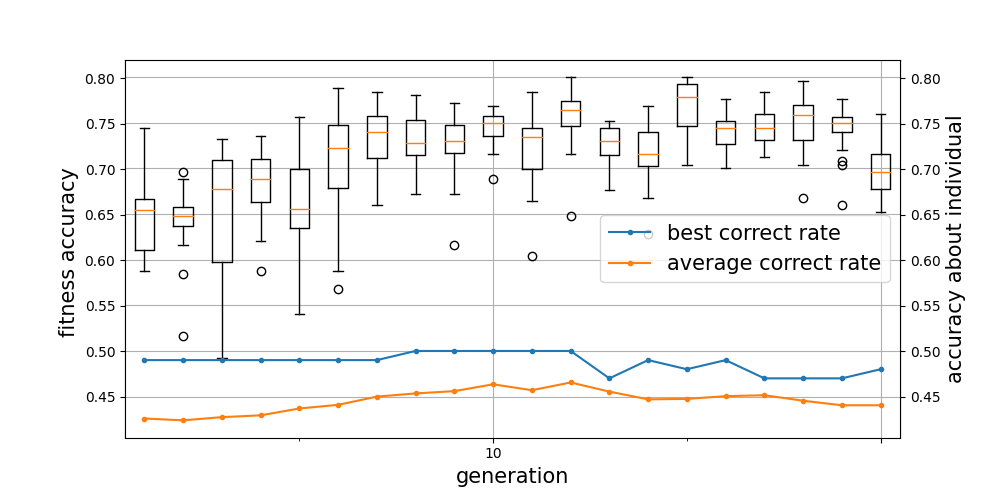
\includegraphics[scale=4.3]{./images/ex1_res_graph.png}
		\caption{実験1 : GA の探索結果\label{fig:ex1_res1}}
	\end{center}
\end{figure}
\clearpage

\begin{figure}[h]
	\begin{center}
		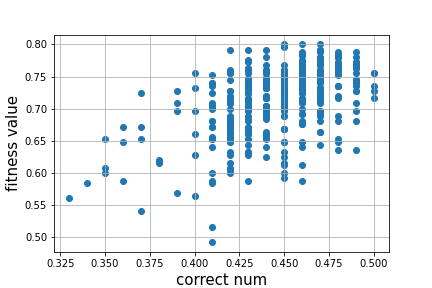
\includegraphics[scale=1.0]{./images/ex1_res_img.png}
		\caption{実験1 : 探索個体の散布図\label{fig:ex1_res2}}
	\end{center}
\end{figure}
\clearpage

次に,表\ref{tb:ex1_res3}に探索された個体によるテスト識別率を示す.
図\ref{fig:ex1_res1}より適応度の平均が最大であった15世代の全個体のうち各遺伝子座で最も多く選ばれた遺伝子を採択して
得られる新たな個体を最終的な個体として学習を行った.またある遺伝子座について選ばれた遺伝子が14世代の全個体に対して占めた割合に対し確信度として閾値を設けて,採択数を絞った状態での学習も行った.

結果は全て探索した疑似ラベルを使用しないベースラインを下回った.
考えられることとして,まず疑似ラベルの精度が低いことによって疑似ラベルによる正則化がうまく機能しなかったことが
挙げられる.また,FixMatch のラベルなしデータによる疑似ラベルの正則化と,ラベル付きデータとして混ぜられた疑似ラベルの正則化が互いに妨害をした可能性が考えられる.

\begin{table}[h]
	\centering
	\caption{実験1 : テスト識別率\label{tb:ex1_res3}}
	\scalebox{1.0}{
		\begin{tabular}{|c|c|c|c|} \hline
			閾値&採択数&正答数&テスト識別率\\ \hline
			&0&&0.868\\ \hline\hline
			なし&100&46&0.836\\ \hline
			0.19&39&22&0.862\\ \hline
			0.2&19&14&0.825\\ \hline
		\end{tabular}
	}
\end{table}

\changeindent{0cm}
\subsection{実験2}
\changeindent{2cm}

表\ref{tb:ex2_data},\ref{tb:ex2_GApara},\ref{tb:ex2_SimCLRpara}にそれぞれ実験2における
各種設定を示す.また,事前学習は SimCLR の Encoder 部のみとし,Classifier の初期重みはランダムなものとした.

\begin{table}[h]
	\centering
	\caption{実験2 : データ内訳\label{tb:ex2_data}}
	\scalebox{1.0}{
		\begin{tabular}{|c||c|} \hline
			$D_{\rm l}$&50\\ \hline
			$D_{\rm ul}$&49850\\ \hline
			$D_{\rm s}$&100\\ \hline
			$D_{\rm t}$&10000\\ \hline
		\end{tabular}
	}
\end{table}


\begin{table}[h]
	\centering
	\caption{実験2 : GAの設定\label{tb:ex2_GApara}}
	\scalebox{1.0}{
		\begin{tabular}{|c|c|} \hline
			個体数&50\\ \hline
			世代数&100\\ \hline\hline
			選択&エリート + トーナメント\\ \hline
			エリート数&2\\ \hline
			トーナメントサイズ&2\\ \hline\hline
			交叉&一様交叉\\ \hline
			個体の交叉率&1.0\\ \hline
			遺伝子座ごとの交叉率&0.5\\ \hline\hline
			突然変異&ランダム遷移\\ \hline
			遺伝子座ごとの突然変異率&0.1\\ \hline
		\end{tabular}
	}
\end{table}


\begin{table}[h]
	\centering
	\caption{実験2 : SimCLR の設定\label{tb:ex2_SimCLRpara}}
	\scalebox{1.0}{
		\begin{tabular}{|c|c|c|} \hline
			model&Encoder&ResNet18\\ \cline{2-3}
			&Projection head&2層MLP(shape:2048to512)\\ \cline{2-3}
			&classifer&MLP(shape:2048to10)\\ \hline\hline
			\multicolumn{3}{|c|}{事前学習}\\ \hline
			train data&unlabeled&50000(:$D_{\rm l}+D_{\rm ul}+D_{\rm s}$)\\ \hline
			batch size&\multicolumn{2}{|c|}{1024}\\ \hline
			epochs&\multicolumn{2}{c|}{500}\\ \hline
			optimizer&\multicolumn{2}{c|}
			{RAdam(lr=$1.0*10^{-3}$)}\\ \hline\hline
			\multicolumn{3}{|c|}{GAの評価}\\ \hline
			train data&labeled&100(:$D_{\rm s}$)\\ \hline
			batch size&\multicolumn{2}{|c|}{16}\\ \hline
			epochs&\multicolumn{2}{c|}{25}\\ \hline
			loss&\multicolumn{2}{|c|}{Cross Entropy Loss}\\ \hline
			optimizer&\multicolumn{2}{c|}{Adam(lr=$5.0*10^{-3}$,momntum=$1.0*10^{-6}$)}\\ \hline
			validation data&\multicolumn{2}{c|}{50(:$D_{\rm l}$)}\\ \hline
			\multicolumn{3}{|c|}{探索された個体の評価}\\ \hline
			train data&labeled&150(:$D_{\rm l}+D_{\rm s}$)\\ \hline
			batch size&\multicolumn{2}{|c|}{16}\\ \hline
			epochs&\multicolumn{2}{c|}{100}\\ \hline
			loss&\multicolumn{2}{|c|}{Cross Entropy Loss}\\ \hline
			optimizer&\multicolumn{2}{c|}{Adam(lr=$1.0*10^{-3}$,momntum=$1.0*10^{-6}$)}\\ \hline
			test data&\multicolumn{2}{c|}{10000(:$D_{\rm t}$)}\\ \hline
		\end{tabular}
	}
\end{table}
\clearpage

\changeindent{0cm}
\subsubsection{結果と考察}
\changeindent{2cm}
図\ref{fig:ex2_res1},\ref{fig:ex2_res2}に GA の探索結果を示す.
図\ref{fig:ex2_res1}は横軸が GA の世代,縦軸は箱ひげ図が適応度,折れ線グラフは疑似ラベルの正答率で,図\ref{fig:ex2_res2}は横軸が疑似ラベルの正答率で縦軸が適応度を示している.
図\ref{fig:ex2_res2}から正の強い相関性があることが確認でき相関係数は0.822である.
また,図\ref{fig:ex2_res1}では適応度,疑似ラベルの正答率ともに上昇していることから,当然ではあるが,ラベル付きデータの精度と学習されたモデルの識別率は強い相関関係があることが分かる.一方で,疑似ラベルの精度は0.37と低い値に収まっており,探索空間が膨大なために局所解に陥った可能性が考えられる.


\begin{figure}[h]
	\begin{center}
		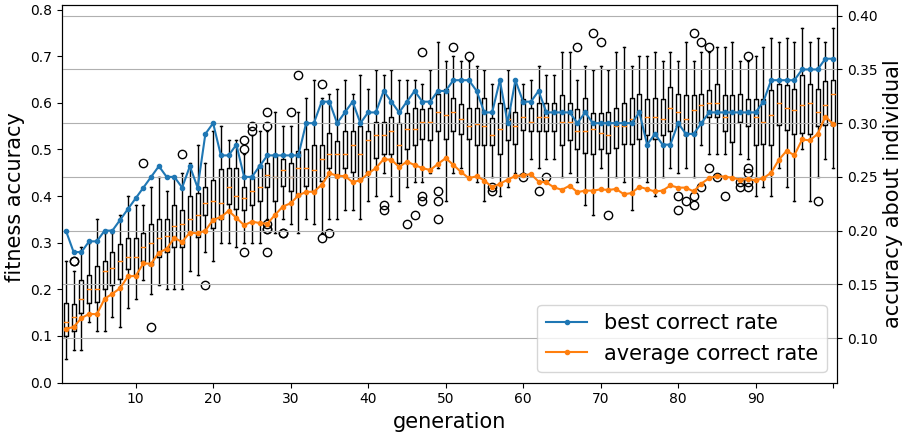
\includegraphics[scale=0.70]{./images/ex2_res_graph.png}
		\caption{実験2 : GA の探索結果\label{fig:ex2_res1}}
	\end{center}
\end{figure}


\begin{figure}[h]
	\begin{center}
		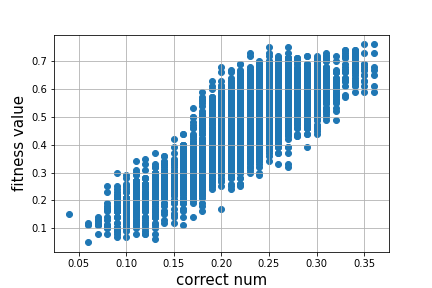
\includegraphics[scale=1.0]{./images/ex2_res_img.png}
		\caption{実験2 : 探索個体の散布図\label{fig:ex2_res2}}
	\end{center}
\end{figure}


次に,表\ref{tb:ex2_res3}に探索された個体によるテスト識別率を示す.
結果は提案手法による疑似ラベルがベースラインおよび
従来の疑似ラベルよりもテスト識別率が劣っていることがわかる.疑似ラベルの精度が低いため
テスト識別率の精度も低くなっていると考えられる.

\begin{table}[h]
	\centering
	\caption{実験2 : テスト識別率\label{tb:ex2_res3}}
	\scalebox{0.8}{
		\begin{tabular}{|c|c|c|} \hline
			$D_{\rm s}$ に対するラベル&テスト識別率&正答率\\ \hline\hline
			正解ラベル&0.822&1.00\\ \hline
			提案手法による疑似ラベル&0.674&0.37\\ \hline\hline
			baseline モデルによる疑似ラベル&0.784&0.74\\ \hline\hline
			baseline (ラベル付きデータのみ)&0.772&$\backslash$\\ \hline
		\end{tabular}
	}
\end{table}

また,実験2では Encoder の学習時間が 1 GPU days かかってはいるものの,
1個体の適応度を出す時間について,実験1に対し16倍ほど速くすることができ,
個体数や世代数を多くするにはベースモデルとして FixMatch よりも SimCLR を用いる方が良いことが分かる.
